\chapter{Test}
I udarbejdelsen af projektet har der været et fokus på at teste systemet, så det hele tiden har blevet verificeret at systemet havde den ønskede funktionalitet. I dette afsnit beskrives testingen af systemet, men for mere information omkring emnet henvises til dokumentationen.
Systemet er blevet testet vha. unit test på de forskellige controllere, opsætning af continues integration og manuelle tests.

\section{Unit tests}
Systemets unit tests er blevet udarbejdet med brug af NUnit og NSubstitute, som begge er test framework til .Net. Unittestene er skrevet i et separat projekt, så det ikke påvirkede projektet.
Unittestene er generelt blevet skrevet på controllers for at verificere, at disse returnerer de rigtige views og kalder rigtigt ned i f.eks. databasen eller ud i andre klasser. Tests i forbindelse med databasen er primært gjort mulige, da vi har anvendt repository pattern. For en uddybende forklaring af dette henvises til dokumentationen \footnote{Se Dokumentation afsnit (Et eller andet)}.

\section{Manuelle tests}
Da det, med det valgte design af applikationen, ikke har været muligt at automatisere alle tests, har disse været suppleret meget med manuelle tests. Dette har på simpel vis foregået ved at en bruger har klikket rundt på hjemmesiden og bekræftet om den nyimplementerede funktionalitet har virket. Dette har eksempelvis været tilfældet når et bytteflow, som kan ses på figur \ref{fig:bytteflow} har fundet sted, hvor en bruger har klikket igennem dette flow og be- eller afkræftet om dette virker efter hensigten.

\begin{figure}[H]
	\centering
	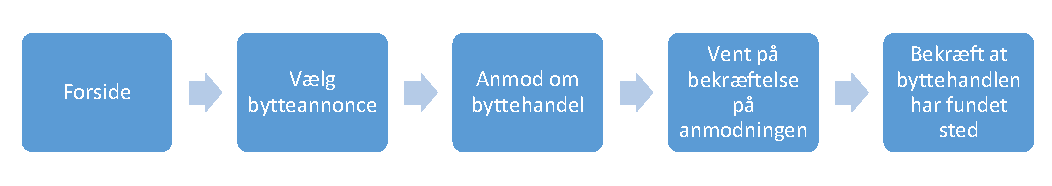
\includegraphics
	[width=140mm]{figures/bytteflow.pdf}
	\caption{Flow over en byttehandel i BargainBarter}
	\label{fig:bytteflow}
\end{figure}

\section{Continuous integration}
Continuous integration blev sat op ved brug af TeamCity. TeamCity-sereven blev sat op til at overvåge gruppens github-repository, så hvert push til repositoriet medførte et build på TeamCity serveren. På TeamCity var to builds sat op i en pipeline. Det første build byggede projektet. Hvis det første build lykkedes, blev det andet build kørt. Dette build kørte alle de tilhørende test til projektet ved brug af et indbygget NUnit-plugin i TeamCity. På baggrund af testene genererer TeamCity en rapport, der indeholder resultatet af de kørte test, samt coverage-analyse, der belyste, hvor stor en del af koden testene dækkede.

I gennem disse redskaber har gruppen opnået erfaringer om hvordan man laver et testbart design. Det har vist sig at controllers der interagerer med brugerprofiler har været svære at teste igennem automatiseret tests, og derfor har der måttes tys til manuelle tests i disse tilfælde. En stor del af projektet har med interaktion af brugerprofiler at gøre og derfor ville det have været prisværdigt at kunne automatisere dette. Dette kunne i projektet have været opnået ved at adskille forretningslogikken fra controllers for på denne måde at lave meget simple controllers der udelukkende stod for interaktion mellem views og database, og udover dette uddelegerede forretningsspecifikke handlinger til en separat klasse. En illustration af dette kan ses på figur \ref{fig:businesslogik}.

\begin{figure}[H]
	\centering
	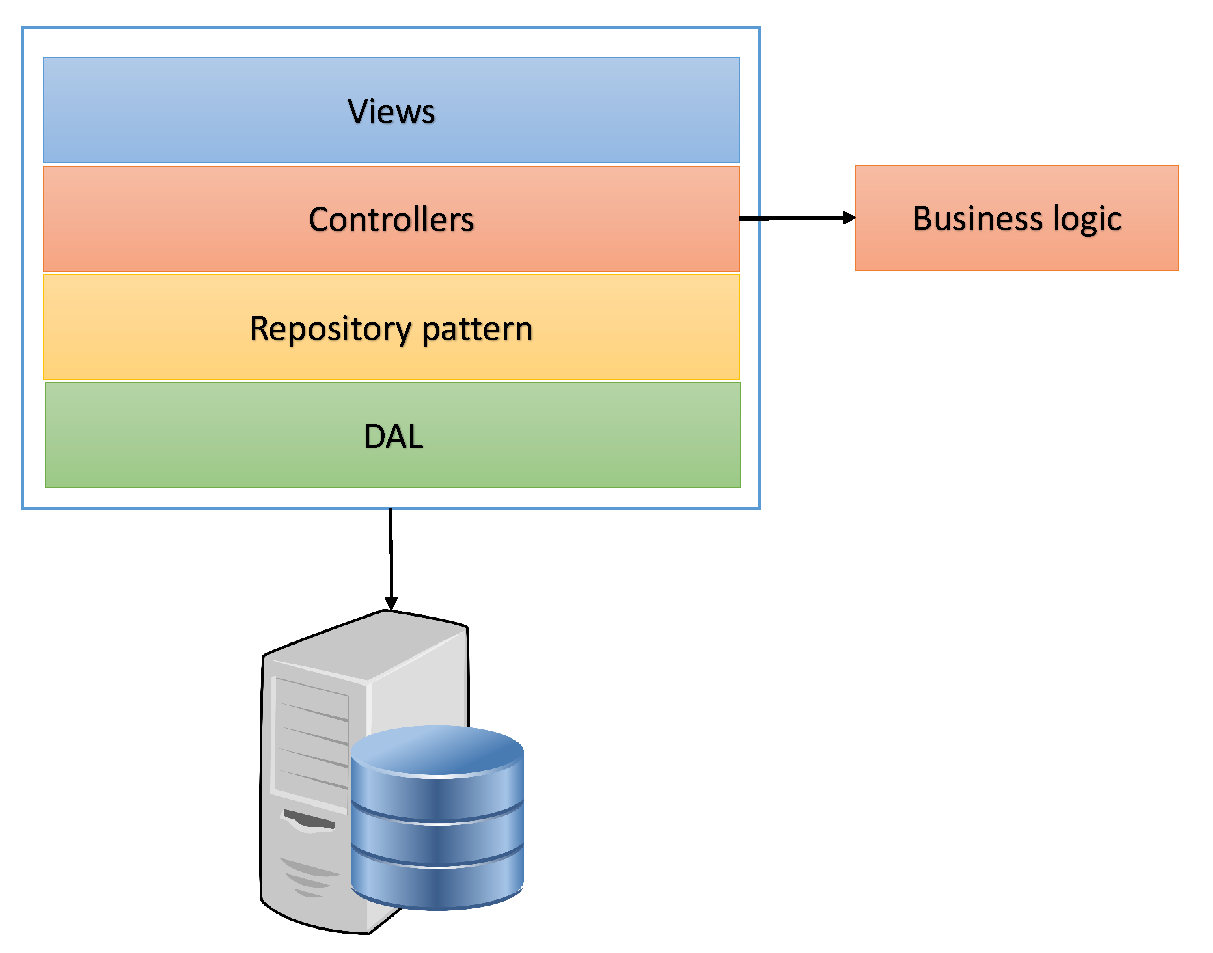
\includegraphics
	[width=140mm]{figures/businesslogik.pdf}
	\caption{Illustration af udvidet design til BargainBarter}
	\label{fig:businesslogik}
\end{figure}

Denne klasse ville så lettere kunne testes for om forretningslogikken har virket.